\chapter{Holes in history space and their arithmetic activation}\label{ch:topology}

When does the history complex $K_A$ of a SELECT-II piece have a two-dimensional hole, and how does divisibility of the source switch it on and off? This is the central arithmetic discovery of the programme: \emph{divisibility acts on topology}. The method is certificate-based. A hole is exhibited by a pair (cycle, cocycle), and survival along the divisibility filtration is decided by which three-dimensional cells are present.

\section{Cycles, cocycles and what can change \texorpdfstring{$H_2$}{H2}}
Let $X=K_A$ with cellular chains $C_j(X)$ over $\F$ spanned by the $j$-faces and boundary $\partial_j$ (the boundary of an ordered partition is the sum of the refinements splitting one block into an ordered pair $(S|T)$). A $2$-\emph{cycle} is $z\in C_2$ with $\partial_2z=0$; a $2$-\emph{cochain} is a linear functional $\varphi$ on $C_2$.
\begin{definition}[hole certificate]\label[definition]{def:certificate}
A \emph{$2$-hole certificate} for $X$ is a pair $(z,\varphi)$ with $\partial_2z=0$, $\varphi(\partial_3c)=0$ for every $3$-face $c$ of $X$, and $\varphi(z)=1$.
\end{definition}
\begin{lemma}\label[lemma]{lem:certificate}
If $(z,\varphi)$ is a $2$-hole certificate for $X$ then $[z]\ne0$ in $H_2(X;\F)$; in particular $\beta_2(X)\ge1$. The check is elimination-free: it needs only $\partial_2z$, the values of $\varphi$ on the boundaries of $3$-faces, and $\varphi(z)$.
\end{lemma}
\begin{proof}
If $z=\partial_3c$ for a $3$-chain $c$ then $\varphi(z)=\sum_{F\in c}\varphi(\partial_3F)=0\ne1$.
\end{proof}
Since $\beta_2=f_2-\rho_2-\rho_3$ and $\partial_3$ maps $3$-faces to $2$-faces, $\beta_2$ depends only on faces of dimension $\le3$ (\cref{thm:face-threshold}(c)). Along the filtration a class created by new $2$-faces therefore survives until new $3$-faces enlarge the image of $\partial_3$ enough to kill it.
\begin{proposition}[what can change $H_2$]\label[proposition]{prop:H2-low}
For a cover $X\subseteq X'$ that creates no $2$-face, $\Delta f_2=0$, $\Delta\rho_2=0$ and $\Delta\beta_2=-\Delta\rho_3\le0$: $\beta_2$ can only decrease, and only through new $3$-faces.

\end{proposition}
\begin{proof}
Extra edges add zero columns to the $2$-face/edge incidence matrix and the row set is unchanged, so $\rho_2$ is unchanged; added $3$-faces can only enlarge the row space of $\partial_3$.
\end{proof}

\section{The anchor cycle}
The two \emph{anchor contents} are $\lambda_A=(2,3,4,5,8,9)$ at source $288$ and $\lambda_B=(2,3,6,7,8,9)$ at source $432$. In rank coordinates $0,\dots,5$ they carry the \emph{same} combinatorial certificate.
\begin{definition}[anchor cycle and cocycle]\label[definition]{def:anchor}
Let $z\subset P_6$ be the sum of $96$ two-faces ($64$ squares and $32$ hexagons, with $130$ vertices) listed in \cref{app:certs}, and let $\varphi$ be the indicator of the six hexagons $(\{2,4,5\}\,|\,\sigma)$, $\sigma$ an ordering of $\{0,1,3\}$ (six faces of type $(3,1,1,1)$).
\end{definition}
The following finite facts are the combinatorial content; the full listing of $z$ and of the objects below is in \cref{app:certs}.
\begin{lemma}[PS-0: combinatorial facts; computer-assisted]\label[lemma]{lem:PS0}
(i) $\partial_2z=0$ and $\varphi(z)=1$. (ii) Among the $540$ three-faces of $P_6$ exactly six have $\varphi(\partial F)=1$: the truncated octahedra $T_a$ and $T_a'$, i.e. $(\{a,2,4,5\}\,|\,y\,|\,w)$ with $a\in\{0,1,3\}$ and $(y,w)$ the two orderings of $\{0,1,3\}\setminus\{a\}$. (iii) The set $P_z=\bigcup_{F\in\operatorname{supp}z}\Pref(F)$ has $43$ proper prefix sets, and for each $a$ the two octahedra $T_a,T_a'$ have the same set $G_a=\Pref(T_a)\setminus P_z$, the \emph{gate} of $a$:
\[
G_0=\{024\},\qquad G_1=\{15,125\},\qquad G_3=\{3,34,35,345\}
\]
(rank sets written as strings).

\end{lemma}
For a content $\lambda$ put $K_z(\lambda)=\operatorname{lcm}_{I\in P_z}D(I)$ (computed on ranks). The six octahedra have thresholds $K_{T_a}=\operatorname{lcm}(K_z,D(I):I\in G_a)$. For the anchors exact computation gives $K_z(\lambda_A)=288$ with $K_{T_a}=576,\,864,\,1440$ for $a=0,1,3$ (i.e. $288\cdot\{2,3,5\}$), and $K_z(\lambda_B)=432$ with $K_{T_a}=864,\,1296,\,3024$ ($432\cdot\{2,3,7\}$). In arithmetic terms the gates are \emph{valuation thresholds} (\cref{prop:valuation}): for $\lambda_A$, $D(024)=2^6$, $D(15)=D(125)=3^3$, $D(3)=5$, so gate $0$ opens when $2^6\mid m$, gate $1$ when $3^3\mid m$ and gate $3$ when $5\mid m$, at the base $m=288=2^5\cdot3^2$; for $\lambda_B$, $D(024)=2^5$, $D(125)=3^4$, $D(3)=7$.

\section{Parametric hole survival}
\begin{theorem}[parametric hole survival; analytic given the finite lemma]\label[theorem]{thm:hole-survival}
Let $\lambda=(c_0<\dots<c_5)$ be \emph{any} six distinct positive integers and $m\ge1$. If $K_z(\lambda)\mid m$ and for each $a\in\{0,1,3\}$ some $I\in G_a$ has $D(I)\nmid m$ (``gate $a$ is closed''), then $[z]\neq0$ in $H_2(X_\lambda(m);\F)$; in particular $\beta_2\ge1$. Equivalently, $z$ survives unless some gate is open ($D(I)\mid m$ for all $I\in G_a$).

\end{theorem}
\begin{proof}
\emph{$z\subset X_\lambda(m)$.} By \cref{thm:face-threshold} a face is present iff all its prefix sets are feasible. Each face of $\operatorname{supp}z$ has $\Pref(F)\subseteq P_z$, and $K_z\mid m$ gives $D(I)\mid m$ for all $I\in P_z$; so the $96$ faces and their subfaces are present, and $z$ is a cycle by \cref{lem:PS0}(i).
\emph{$\varphi\circ\partial_3=0$ on $C_3(X_\lambda(m))$.} By \cref{lem:PS0}(ii) $\varphi(\partial F)=0$ for every $3$-face of $P_6$ except the six octahedra. If one of them, say with first block $\{a,2,4,5\}$, were present then $\Pref(T)\subseteq\mathfrak F_\lambda(m)$; since $\Pref(T)\setminus P_z=G_a$ this makes gate $a$ open, contradicting the hypothesis.
\emph{Conclusion.} $\varphi(z)=1$, so $(z,\varphi)$ is a certificate (\cref{lem:certificate}).
\end{proof}
\begin{proposition}[existence of a surviving regime]\label[proposition]{prop:existence-survival}
A content $\lambda$, with a role bijection $\sigma\in S_6$ applied to the ranks of $z$, admits a source $m$ with $[z_\sigma]\ne0$ via \cref{thm:hole-survival} iff every gate of $\sigma$ contains a set $I$ with $D(\sigma I)\nmid K_z^\sigma(\lambda)$. In that case $m=K_z^\sigma(\lambda)$ is extremal.

\end{proposition}
\begin{proof}
If $m$ works then $K_z\mid m$ and each gate has a set with $D(I)\nmid m$; as $K_z\mid m$, $D(I)\nmid K_z$ as well. Conversely $m=K_z$ satisfies both hypotheses.
\end{proof}
\begin{corollary}[anchor obstruction; survival analytic, fillings finite-exact]\label[corollary]{thm:anchor}
For $\lambda_A$: $z$ is non-bounding in $X(m)$ whenever $288\mid m$ and $576,864,1440\nmid m$, equivalently $288\mid m$ and $\gcd(m/288,30)=1$. For $\lambda_B$ the same holds with $432$ and $\gcd(m/432,42)=1$. Moreover the six octahedra are the only $3$-faces obstructing $z$, with thresholds $288\cdot\{2,3,5\}$ and $432\cdot\{2,3,7\}$. In the opposite direction, for each of the $55$ (resp.\ $59$) regimes of $\lambda_A$ (resp.\ $\lambda_B$) the second Betti number is computed exactly: $\beta_2>0$ only at the single regimes of $288$ and $432$, and whenever $288\mid m$ and one of $576,864,1440$ divides $m$, $z$ bounds, with explicit verified $3$-chain fillings of $34$, $52$ and $126$ faces.

\end{corollary}

\begin{figure}[ht]\centering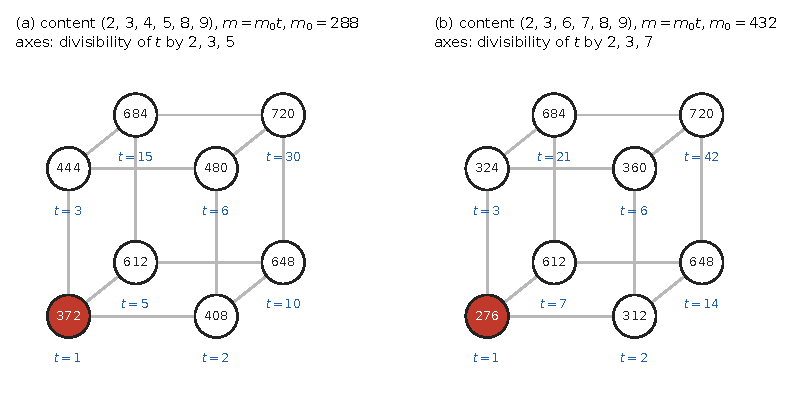
\includegraphics[width=\textwidth]{figures/fig_activation_cube.pdf}
\caption{The eight regimes of the comparable window form a Boolean cube indexed by which gate primes divide $t$ in $m=m_0t$, with history counts $N$ (exact). The hole of the anchor survives only at the bottom vertex $t$ coprime to the gate primes (red); multiplying by any gate prime fills it, and the filled state is absorbing under divisibility. Left: $\lambda_A$, $m_0=288$, gates $2,3,5$. Right: $\lambda_B$, $m_0=432$, gates $2,3,7$, where the vertex for $3\cdot7$ carries the interaction $+24$ of \cref{obs:counting}.}\label{fig:cube}
\end{figure}
\begin{figure}[ht]\centering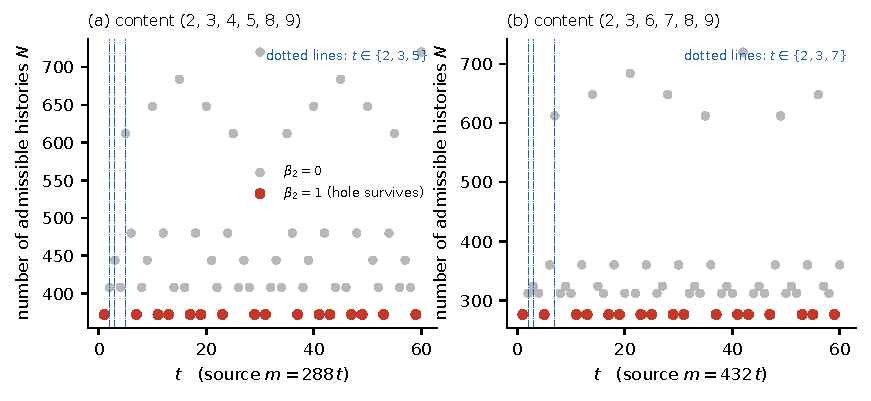
\includegraphics[width=\textwidth]{figures/fig_activation_series.pdf}
\caption{Divisibility activation along $m=288t$ and $m=432t$, $t=1,\dots,60$: the history count $N$ (exact, from the admissible-set simulation) with the sources at which the hole survives in red. Survival occurs exactly for $t$ coprime to $30$ (a) and to $42$ (b); dotted lines mark the gate primes at which a gate opens and the hole is filled.}\label{fig:activation}
\end{figure}

\section{The exact survival criterion}
\Cref{thm:hole-survival} is a sufficient condition phrased through gates. All $3$-faces of $P_6$ have $\Pref(F)\subseteq P_z\cup\mathrm{EXTRA}$, where $\mathrm{EXTRA}$ is a set of $20$ further prefix sets (listed in \cref{app:certs}). Whether $z$ bounds in $X_\lambda(m)$ with $K_z\mid m$ therefore depends only on $S=\mathfrak F_\lambda(m)\cap\mathrm{EXTRA}$, and is a monotone Boolean function of $S$: more feasible sets give more $3$-faces.
\begin{theorem}[exact survival criterion; finite-exact]\label[theorem]{thm:exact-survival}
For $K_z\mid m$: $[z]=0$ in $H_2(X_\lambda(m);\F)$ iff $S$ contains one of the four minimal families
\[
B_0=\{024\},\quad B_1=\{15,125,1235\},\quad B_2\ (15\text{ sets}),\quad B_3\ (17\text{ sets}),
\]
(the last two listed in \cref{app:certs}); equivalently $[z]\ne0$ iff $K_z\mid m$ and $S$ contains none of $B_0,\dots,B_3$. Exactly $589{,}839$ of the $2^{20}$ families bound. The criterion is a statement about $P_6$ alone and holds for every content. \Cref{thm:hole-survival} is a corollary: every $B_i$ contains a full gate ($G_0\subseteq B_0$, $G_1\subseteq B_1$, $G_3\subseteq B_2,B_3$), so ``every gate has a closed set'' excludes all four.

\end{theorem}
\begin{remark}[the naive gate condition is not necessary]\label[remark]{rem:gate-correction}
A natural \emph{bounded-negative} statement, observed without exception on $18{,}980$ regimes with labels $\le16$, is that if gate $1$ or gate $3$ is open then $z$ bounds. \Cref{thm:exact-survival} refutes it as a general statement: $B_1$ contains the gate $G_1=\{15,125\}$ \emph{and} the further set $\{1235\}$, and $B_2,B_3$ contain $G_3$ together with many more sets, so a regime in which a gate is open but the remaining sets are infeasible still carries a hole. Gate $0$ is the exception: $B_0=G_0$ is a singleton, so opening gate $0$ always kills $z$ (the universal filling).
\end{remark}
\begin{proposition}[gate necessity fails; finite-exact]\label[proposition]{prop:gate-nec}
There are contents and sources with gate $1$ open (resp.\ gate $3$ open) in which $[z]\ne0$: for gate $1$, labels $(634404,\,1566830,\,1769151,\,2255330,\,3302454,\,3302705)$; for gate $3$, labels $(906654,\,921305,\,1769151,\,2255330,\,3574704,\,4433330)$, each with the source recorded in the certificate. The small-label census missed them only because small labels cannot realise the required prime patterns.

\end{proposition}
\begin{proposition}[realisation by the Chinese remainder theorem]\label[proposition]{prop:CRT}
For an odd prime $p$ the weight $\omega_p(r)$ of a label can be prescribed independently for the six ranks as any element of $\{0,1,2,\dots\}\cup\{-2,-4,\dots\}$: a weight $v\ge1$ by $c_r\equiv p^v\ (\mathrm{mod}\ p^{v+1})$, a weight $-2v$ by $c_r\equiv-p^v\ (\mathrm{mod}\ p^{v+1})$, weight $0$ by a residue mod $p$ that is neither $0$ nor $-1$. By CRT the residues for distinct primes can be chosen simultaneously. Hence any intersection of single-prime masks $\{I:\omega_p(I)\le v_p(m)\}$ is realised as $\mathfrak F_\lambda(m)$ restricted to the prefix sets that matter, provided the additional prime factors of the labels (which only add constraints at other primes) are absorbed by taking $m$ equal to the lcm of the needed denominators.

\end{proposition}

\section{The six-label census}
\begin{observation}[six-label census of $H_2$; finite-exact]\label[observation]{obs:census-H2}
Over all $8{,}008$ six-label contents with labels in $\{1,\dots,16\}$ and all $346{,}859$ of their source regimes, $158$ regimes have $\beta_2>0$ ($157$ with $\beta_2=1$ and one, content $(2,3,8,9,14,15)$ at source $1680$, with $\beta_2=3$). Of these, $52$ are explained by \cref{thm:hole-survival} for some role bijection; $106$ are not and carry other $H_2$ patterns (thirty-three coarse signatures; the most common has a $50$-face cycle and four obstructed truncated octahedra). Forty-six contents admit a regime of the first kind. Among $18{,}998$ regimes with $z\subset X$, $18$ satisfy the hypotheses of \cref{thm:hole-survival} and all $18$ have $[z]\ne0$; in the other $18{,}980$ some gate is open and $z$ bounds in every case.

\end{observation}
This is a statement about a census. It does not say that the census exhausts the mechanisms of $H_2$ (\cref{ch:atlas}), nor that labels $\le16$ exhibit gate necessity (they do not, by \cref{prop:gate-nec}). The \emph{role-permutation} caveat is essential: the identity role map (the cycle placed on ranks as given) detects only some regimes, and applying $\sigma\in S_6$ to the cycle gives different families, so a count for the ``anchor class'' must say which role maps it ranges over (see also \cref{obs:rolemap}).
